\documentclass[a4paper, 12pt, english]{article}

\usepackage[utf8]{inputenc}
\usepackage{amsmath,amssymb}
\usepackage{graphicx}
\usepackage{subfig}

\usepackage{indentfirst}
\usepackage{verbatim}
\usepackage{textcomp}

\usepackage{tabularx}

\usepackage{relsize}

%for rendering code
\usepackage{minted}


%for drawing phazors
\usepackage{tikz}

%for fancy numbers
\usepackage{siunitx}

%for floating tables 
\usepackage{float}

%for roman numbering
\usepackage{romannum}

%for degree and other generic symbols
\usepackage{gensymb}

%for bottom numbering
\pagenumbering{arabic}


%creates myrule command to create a line
\NewDocumentCommand{\myrule}{O{1pt} O{2pt} O{black}}{%
  \par\nobreak % don't break a page here
  \kern\the\prevdepth % don't take into account the depth of the preceding line
  \kern#2 % space before the rule
  {\color{#3}\hrule height #1 width\hsize} % the rule
  \kern#2 % space after the rule
  \nointerlineskip % no additional space after the rule
}

\usepackage[section]{placeins}

\usepackage{booktabs}
\usepackage{colortbl}%
   
\usepackage[obeyspaces]{url}
\usepackage{etoolbox}
\usepackage[colorlinks,citecolor=black,urlcolor=blue,bookmarks=false,hypertexnames=true]{hyperref} 

%controls margins and paper size
\usepackage{geometry}
\geometry{
	paper=a4paper, % Change to letterpaper for US letter
	inner=2cm, % Inner margin
	outer=2cm, % Outer margin
	left   = 2cm,
	right  = 2cm,
	marginparsep = 0pt,
	marginparwidth=0pt,
	%bindingoffset=.0cm, % Binding offset
	top=2cm, % Top margin
	bottom=1.5cm, % Bottom margin
	%showframe, % Uncomment to show how the type block is set on the page
}

%for headers and footers
\usepackage{fancyhdr}
\pagestyle{fancy}
\fancyhf{}
%\fancyhead[L]{\textbf{My Lab Report}}
%\fancyhead[R]{\today}
\fancyfoot[L]{EE222}
\fancyfoot[C]{\thepage}
\fancyfoot[R]{Lab Work\#1}
\renewcommand{\headrulewidth}{0pt} % remove the header rule line


%to remove numbers but keep numbering for sections
\makeatletter
% we use \prefix@<level> only if it is defined
\renewcommand{\@seccntformat}[1]{%
  \ifcsname prefix@#1\endcsname
    \csname prefix@#1\endcsname
  \else
    \csname the#1\endcsname\quad
  \fi}
% define \prefix@section
\newcommand \prefix@section{Part \Romannum{\thesection}: }
\makeatother

%************************************START**************************************%
\begin{document}
\pagenumbering{arabic}

%************************************TITLE PAGE**************************************%
\begin{titlepage}
\begin{center}
\textsc{\Large \bfseries People's Democratic Republic of Algeria}\\[0.3cm] 
\textsc{\Large \bfseries Ministry of Higher Education and Scientific Research}\\[0.75cm] 
\textsc{\Large \bfseries Institute of Electrical and Electronic Engineering }\\[0.5cm]

\par
\vspace{20pt}
\textbf{\Large \bfseries EE222 Digital Systems}\\
\vspace{15pt}
\myrule[1pt][10pt]
\vspace{20pt}
\textbf{\LARGE  LABORATORY REPORT \#1}\\
\vspace{20pt}
\textbf{\large Design, Simulation and Implementation of BCD Adders and ALU Using behavioral Modeling}\\
\vspace{15pt}
\myrule[1pt][7pt]
\vspace{25pt}

\textbf {\large Done by:}\\[0.2cm]
\begin{center}
\begin{tabular}{ l }
 AMMOUR Fatma\\
 BOUTITE Ramzi\\
 BOULEGROUN Amin \\  
\end{tabular}
\end{center}


\textbf {\large Group:}
\begin{center}
  L2 Group 08 
\end{center}


\vspace{45pt}
\textbf {\large Instructor:}\\[0.2cm]
 Y.AZZOUGUI\\[0.1cm]
\end{center}

\par
\vfill
\begin{center}
	\textbf{Date:\\}
	\small{19/02/2023}\\
\end{center}
\end{titlepage}


\newpage
\section*{Introduction}
Arithmetic and logical operations are a fundamental building block of processors and controllers. Therefore, it is important to understand how to implement them using VHDL, and how to simulate and test their functionality. 

\section*{Objectives}
The objective of this lab work is to design a one-digit and two-digit BCD adder and an arithmetic and logical unit (ALU) using sequential VHDL programming.

\newpage

\section{One-Digit BCD Adder}
%\lstinputlisting[language=Vhdl, title=First Exercise vhdl code]{part1.vhd}
\subsection{Problem Statement:}
A 1-digit BCD adders outputs the sum of the two BCD digits input, and also considers a carry in and out bit. The problem requires implementing the adder using the IF-ELSE statement.
The design requires 2 BCD digits (4bits $\times$ 2) and a carry-in bit as inputs, and the output is 1 BCD digit and a carry-out bit.
\subsection{Design approach:}
Constructing a BCD adder is based on 2 conditions. If the sum is less or equal to 9, then we perform the addition in a normal fashion. Else, the sum is greater than 9, so we adjust by adding 6 to the sum to complement the base 16 digit into 2 digits of base 10. The second digit can only be 1, so we represent it using the carry-out bit.\\
The codes will utilize the numeric\_std in order to be able to perform different operations.\\
Notice the concatenation of 0 to the beginning of the first input, this is to allocate the extra bit needed for the carry-out.
\subsection{VHDL code:}
%\lstinputlisting[language=Vhdl, title=First Exercise vhdl code]{part1.vhd}
\begin{listing}[H]
\inputminted[linenos,bgcolor=gray!20]{Vhdl}{part1.vhd}
\end{listing}

\subsection{Simulation result:}
For the simulation, we avoided including all cases, since we only need to confirm that it works for both cases.\\
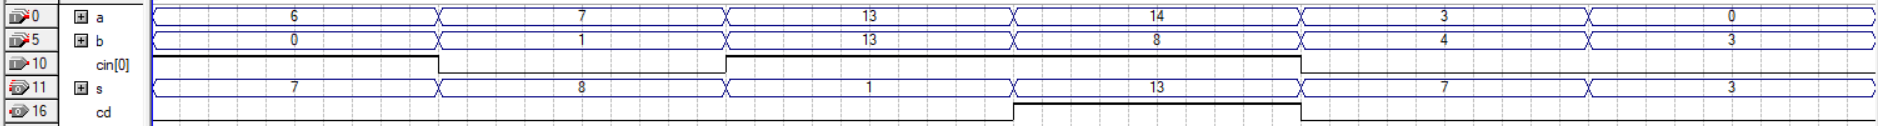
\includegraphics[width=\textwidth]{lab 1/ex1.png}
From the simulation, we notice that it works just as planned, except for when the entered values are out range of a BCD digit. The problem can be solved by adding a condition to confirm that the input digit is less than 10. However for normal cases it should not be a problem.

\newpage
\section{Two-Digit BCD Adder}
\subsection{Problem statement:}
A 2-digit BCD adder outputs the sum of 2 $\times$ 2 BCD digits input and a carry-in bit. The output is a 2 digit BCD, with the carry-out bit. A 2 digit BCD contains 4 $\times$ 2 bits per pair. 
\subsection{Design approach:}
Using the same principle from 1-digit BCD adder, we can combine two of them to make our adder. The first adder will calculate the first digit output from our 2 input digits, then the second digit using the 2nd 2 inputs. While passing the carry-out of first adder into the carry-in of the second adder. And taking the extra resulting third digit as the final carry-out. 

\subsection{VHDL code:}
\inputminted[linenos,bgcolor=gray!20]{Vhdl}{part2.vhd}

\subsection{Simulation result:}
For the simulation, we avoided including all cases again for same previous reason.\\
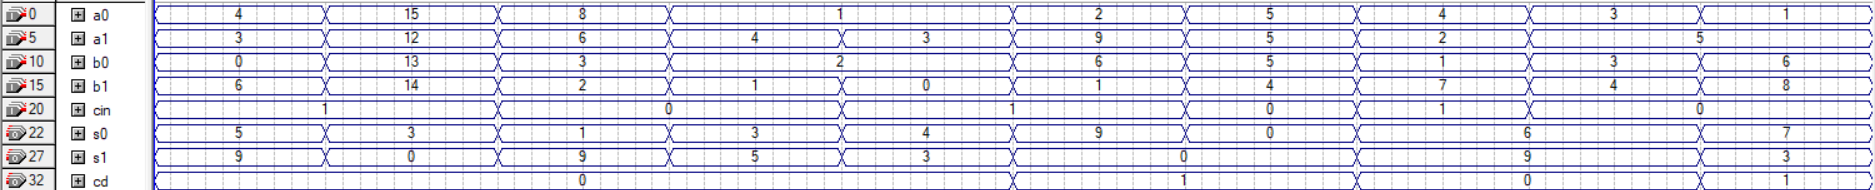
\includegraphics[width=\textwidth]{lab 1/ex2.png}
Since we continued using the same principle from the earlier, the "problem" is still relevant here and can be solved with the same solution.


\newpage
\section{The Arithmetic and logic Unit (ALU):}
\subsection{Problem statement:}
An ALU that can compute various arithmetic and logical operations. It accepts two 4 bits inputs, 4 bits opCode input, and outputs a 4bit result with 3 different flags (negative, zero and carry flag). The output is also passed through a hex to 7-seg decoder.\\
\subsection{Design approach:}
Using CASE-WHEN, we can check for the opCode and return the appropriate operation result to Y. For the hex to 7-seg decoder, we assign the LEDs activation order for each value possible.

\subsection{VHDL code:}
\inputminted[linenos,bgcolor=gray!20]{Vhdl}{ex3.vhd}
\subsection{Simulation result:}
The simulation includes all the operations done on randomly selected values for A and B.
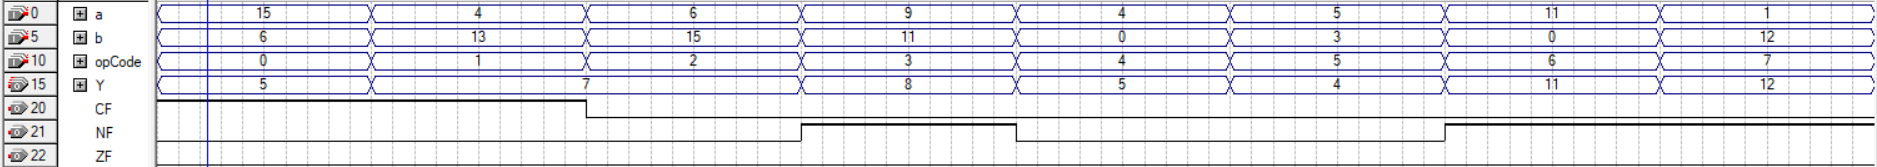
\includegraphics[width=\textwidth]{lab 1/ex3.png}
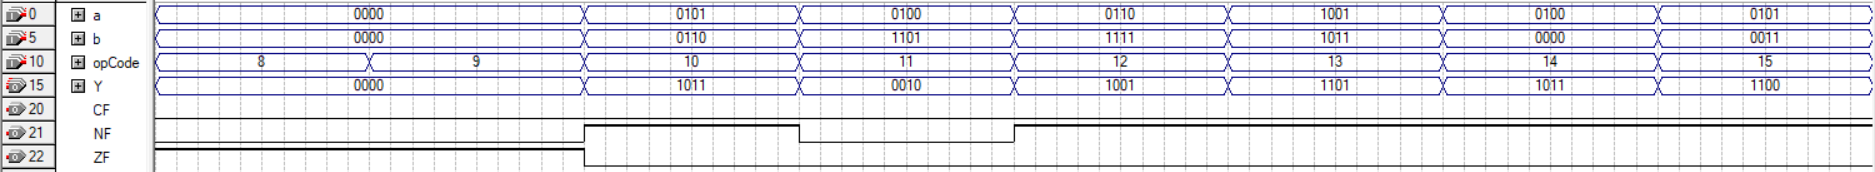
\includegraphics[width=\textwidth]{lab 1/ex3-2.png}
We remark that even though the NF was design for subtraction except that it is activated in the other cases, this is because most of the other cases are logical operations that can invert zeros to ones, thus inverting the "sign bit" from positive 0 to negative 1.
%\subsection{Problem statement:}
%\subsection{Design approach:}
%\subsection{VHDL code:}
%\subsection{Simulation result:}

\newpage
\section*{Conclusion}
In conclusion, this lab work focused on designing and implementing various adders and an ALU using VHDL. The one-digit and two-digit BCD adders were designed and simulated successfully. The ALU was designed to perform various arithmetic and logical operations based on the opcode input with the output hex to 7-seg decoder and was also successful.
\end{document}
